\section{Experiment 2. Within-method interventions}\label{sec:exp2}


\subsection{BO-EI recovery after an early miss}
\label{sec:bo_recovery}
For a GP posterior \(Y(x)\mid\mathcal D_t\sim\mathcal N(\mu_t(x),s_t^2(x))\), expected improvement with offset \(\xi\geq0\) is
\begin{equation}
\label{eq:ei}
 \EI_\xi(x)
 =\mathbb E[(F_t-\xi-Y(x))_+]
 =\delta_t(x)\Phi(z_t(x))+s_t(x)\phi(z_t(x)),
\end{equation}
where \(F_t\) is the best observed objective value,
\(\delta_t(x)=F_t-\xi-\mu_t(x)\),
\(z_t(x)=\delta_t(x)/s_t(x)\), and \(\Phi,\phi\) are the standard normal distribution and density. When \(s_t(x)=0\), EI equals \((\delta_t(x))_+\).

The offset \(\xi\) determines how much improvement is required before an outcome contributes positively to the acquisition. With \(\xi=0\), any improvement over \(F_t\) contributes. With \(\xi>0\), an outcome must improve on \(F_t\) by more than \(\xi\). Near an already explored local minimum, the posterior may predict only small further improvements with little uncertainty. Increasing \(\xi\) makes these evaluations less attractive. Less explored locations with greater posterior uncertainty may still offer a substantial chance of exceeding the larger improvement threshold, making them relatively more attractive.

As derived in \eqref{eq:uniform}, by sampling points via a uniform distribution on the space (we hereby refer this as 'uniform probes'), we have probability \(\pi\rho_c^2/64\) of hitting the discovery circle independently of the posterior. This motivates comparing a change to the acquisition offset with an explicit allocation of evaluations to global sampling.

At each of \(c=10,30\), 50 seeds first run standard BO-EI for 12 evaluations. For evaluations that do not discover the better basin, we copy the historical trajectories into four continuations: standard EI; EI with \(\xi=0.5\); standard EI with ten uniform probes; and the combination. Probes replace EI proposals at evaluations \(13,16,\ldots,40\), with the same probe locations used by both probe variants within a seed. All observations update the GP, and evaluations 41-50 use standard EI in every variant. The comparison between methods therefore measures recovery conditional on an early miss, within the same total budget.

\begin{table}[!htb]
 \centering
 \caption{Discovery / precision counts at evaluation 50 among
 histories with \(F_{12}\geq1\).}
 \label{tab:bo}
 \begin{tabular}{lcc}
 \toprule
 Continuation & \(c=10\), \(n=39\) & \(c=30\), \(n=42\)\\
 \midrule
 Standard BO-EI       & 8/7   & 1/1\\
 \(\xi=0.5\)          & 14/14 & 8/7\\
 Uniform probes      & 27/23 & 21/14\\
 \(\xi=0.5\) + probes & 31/28 & 22/14\\
 \bottomrule
 \end{tabular}
\end{table}

Uniform probes increase discovery by 48.7 percentage points at \(c=10\) (95\% CI \([17.4,69.6]\)) and 47.6 points at \(c=30\) (\([20.2,65.6]\)). Precision also increases, by 41.0 and 31.0 points, with intervals \([13.1,60.1]\) and \([3.7,51.7]\). Increasing \(\xi\) alone gives smaller observed gains, whose intervals include zero. The additional benefit of increasing \(\xi\) is more significant when $c=10$. As the global basin becomes harder to find, the benefits become less significant.

The trajectories support the proposed coverage explanation. During evaluations 13--40, probes increase the mean number of newly visited unit grid cells from 5.0 to 13.6 at \(c=10\) and from 3.4 to 12.8 at \(c=30\). The fraction of evaluations within distance 1 of \(a\) decreases from \(73\%\) to \(36\%\) and from \(85\%\) to \(44\%\). Of the discoveries under standard EI with probes, 9 occur at probes and 18 at EI proposals for \(c=10\); the corresponding counts are 11 and 10 for \(c=30\). Thus the policy can help through both directly reaching the basin or subsequent model-guided evaluations from the discovery-favouring method. 

\begin{figure}[!htb]
 \centering
 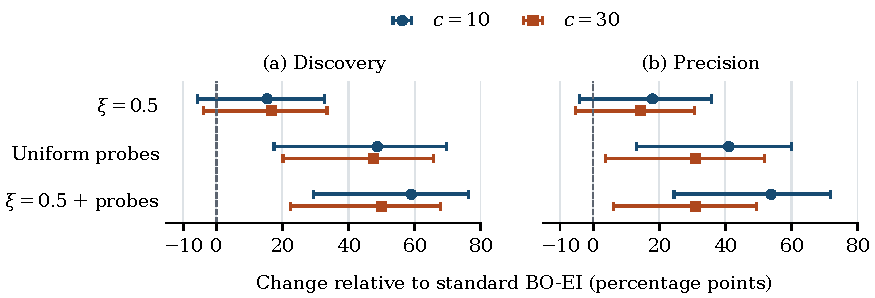
\includegraphics[width=.90\linewidth]{bo_paired_effects.pdf}
 \caption{Paired differences in target-attainment proportions relative to standard BO-EI. Bars show conservative 95\% confidence intervals for individual contrasts.}
 \label{fig:boeffects}
\end{figure}


\subsection{Trust-region contraction and restarts in TuRBO-1}
TuRBO-1 uses Thompson sampling from a local GP posterior within an adaptive trust region centred on the incumbent. The trust region contracts after a specified number of consecutive unsuccessful iterations and restarts when its length falls below a minimum threshold. To investigate whether premature concentration around the inferior basin limits discovery, we vary the normalised initial trust-region length \(L_0\) and failure tolerance \(k_{\rm fail}\). The six variants share four initial design points within each seed, with all 50 seeds per penalty included in the comparison. The configurations differ from the first model-guided proposal onward.

\begin{table}[!htb]
 \centering
 \caption{TuRBO-1 outcomes after 50 evaluations. Each cell reports discovery count / precision count / count of runs with at least one restart, out of 50 runs.}
 \label{tab:turbo}
 \begin{tabular}{lcccc}
 \toprule
 Variant & \(L_0\) & \(k_{\rm fail}\) & \(c=10\) & \(c=30\)\\
 \midrule
 Default               & 0.8 & 4  & \(12/9/30\)  & \(5/4/29\)\\
 Small region          & 0.4 & 4  & \(20/10/45\) & \(11/5/41\)\\
 Large region          & 1.6 & 4  & \(12/10/26\) & \(6/5/24\)\\
 Fast contraction      & 0.8 & 2  & \(19/13/50\) & \(14/9/50\)\\
 Slow contraction      & 0.8 & 8  & \(10/9/0\)   & \(4/3/0\)\\
 Very slow contraction & 0.8 & 12 & \(11/9/0\)   & \(4/3/0\)\\
 \bottomrule
 \end{tabular}
\end{table}

Smaller initial regions and faster contraction improve discovery under the fixed evaluation budget (Table~\ref{tab:turbo}). At \(c=30\), fast contraction increases discovery from 5/50 to 14/50 and precision from 4/50 to 9/50. It also advances the median first restart from evaluation 44 to 28, with all 50 runs restarting compared with 29 under the default configuration. In contrast, both slower-contraction variants record no restarts and only 4/50 discoveries.

The evaluation histories provide further insight into how restarts contribute to discovery. At \(c=30\), nine of the 14 successful fast-contraction runs first discover the better basin after restarting, including seven during the fresh four-point initial design and two during subsequent local search. This suggests that restarts can facilitate discovery both directly through renewed global sampling and indirectly by enabling local search in a new region.

The smaller initial-region variant also improves discovery to 11/50 at \(c=30\), although its median first restart occurs at evaluation 42, only slightly earlier than the default. Of its 11 discoveries, two occur during restart initialisation and four during subsequent local search. Thus, restart timing alone does not fully explain the observed differences; changes in local search trajectories may also contribute.

Overall, these results suggest that abandoning an unpromising trust region and restoring broader exploration can improve TuRBO-1's discovery performance on the two-basin objective. However, the interventions also change the proposals before restarting, so the observed improvements cannot be attributed exclusively to restarts.

\subsection{Effects of population size, parent count, and mean updates
on CMA-ES discovery and precision}

Experiment~1 showed that CMA-ES can discover the better basin without
reaching the precision target. We examine how population size
\(\lambda\), the number of selected parents \(\mu\), and the size of
the mean update affect discovery, precision, and settling near \(b\).
We study settling speed at \(c=3\) and compare discovery and precision
at \(c=30\). In the comparisons reported here, we initialise the search
mean at \((1.8,0)\), \((1.6,0)\), or \((1.4,0)\).
Each configuration uses the same 20 seeds at each starting location,
giving 60 matched seed--offset combinations. We record discovery and
precision for the same runs at 50 and 200 objective evaluations.

We first vary population size and settling speed.
At \(c=3\), we compare CMA-ES populations of 6 and 12, with
\(\mu=\lambda/2\). We pair runs by seed and starting location.
To measure how quickly the search concentrates around \(b\), we use
the root-mean-square (RMS) distance of the sampling distribution to \(b\),
\[
D_b=\sqrt{\|m-b\|_2^2+\operatorname{tr}(\Sigma)},
\]
where \(m\) is the search mean and \(\Sigma\) is the sampling covariance,
both expressed on the original domain. The settling evaluation is the
first evaluation from which \(D_b\) stays below \(0.4\) through
evaluation 200. Among the 37 matched pairs in which both configurations
settled near \(b\), the population of 6 settled sooner in 30 pairs,
tied in four, and settled later in three
(Figure~\ref{fig:cmaes-results}, top row, panel (a)).
Across all 60 runs per configuration, the median RMS distance to \(b\)
generally decreased faster and remained lower for \(\lambda=6\) over
most of the evaluation budget
(Figure~\ref{fig:cmaes-results}, top row, panel (b)).
At evaluation 50, it was \(0.88\) for
\(\lambda=6\) and \(1.36\) for \(\lambda=12\). Both medians were close
to zero by evaluation 200, indicating that the smaller population
typically concentrated around \(b\) sooner. Across all runs,
\(\lambda=12\) finished near \(b\) more often (52 versus 42 runs).
Overall, the smaller population tended to concentrate around \(b\)
sooner, while the larger population finished near \(b\) in more runs.

We then vary parent count at a fixed population size.
With \(\lambda=12\) fixed, the bottom-left plot in
Figure~\ref{fig:cmaes-results} shows that discovery (\(f<1\))
increased as more parents were selected. Precision (\(f<0.01\)) and
the share of runs whose sampling distributions finished near \(b\)
generally decreased, with a slight recovery at the largest parent
count. Since each setting evaluated the same number of candidates
per generation, the difference concerns how those candidates were
used to update the search. For runs starting near \(b\), selecting
more parents favoured discovery, while selecting fewer was associated
with both greater concentration near \(b\) and more precise solutions.

We also halve the mean update.
At \(c=30\), starting near \(b\), the halved mean update outperformed
the standard update on both discovery and precision. In the left plot
of the bottom-right panel of Figure~\ref{fig:cmaes-results},
the discovery curve (\(f<1\)) rises faster and stays above the
standard-update curve once they separate. In the right plot, the
precision curve (\(f<0.01\)) also pulls ahead, and its lead grows as
more evaluations are used. By 200 evaluations, the halved update
achieved discovery in 53 of 60 runs, compared with 44 under the
standard update, and reached precision in 33 runs, compared with 16.
The advantage therefore extended from finding the better basin to
reaching the stricter precision target.

\begin{figure}[!htbp]
\centering
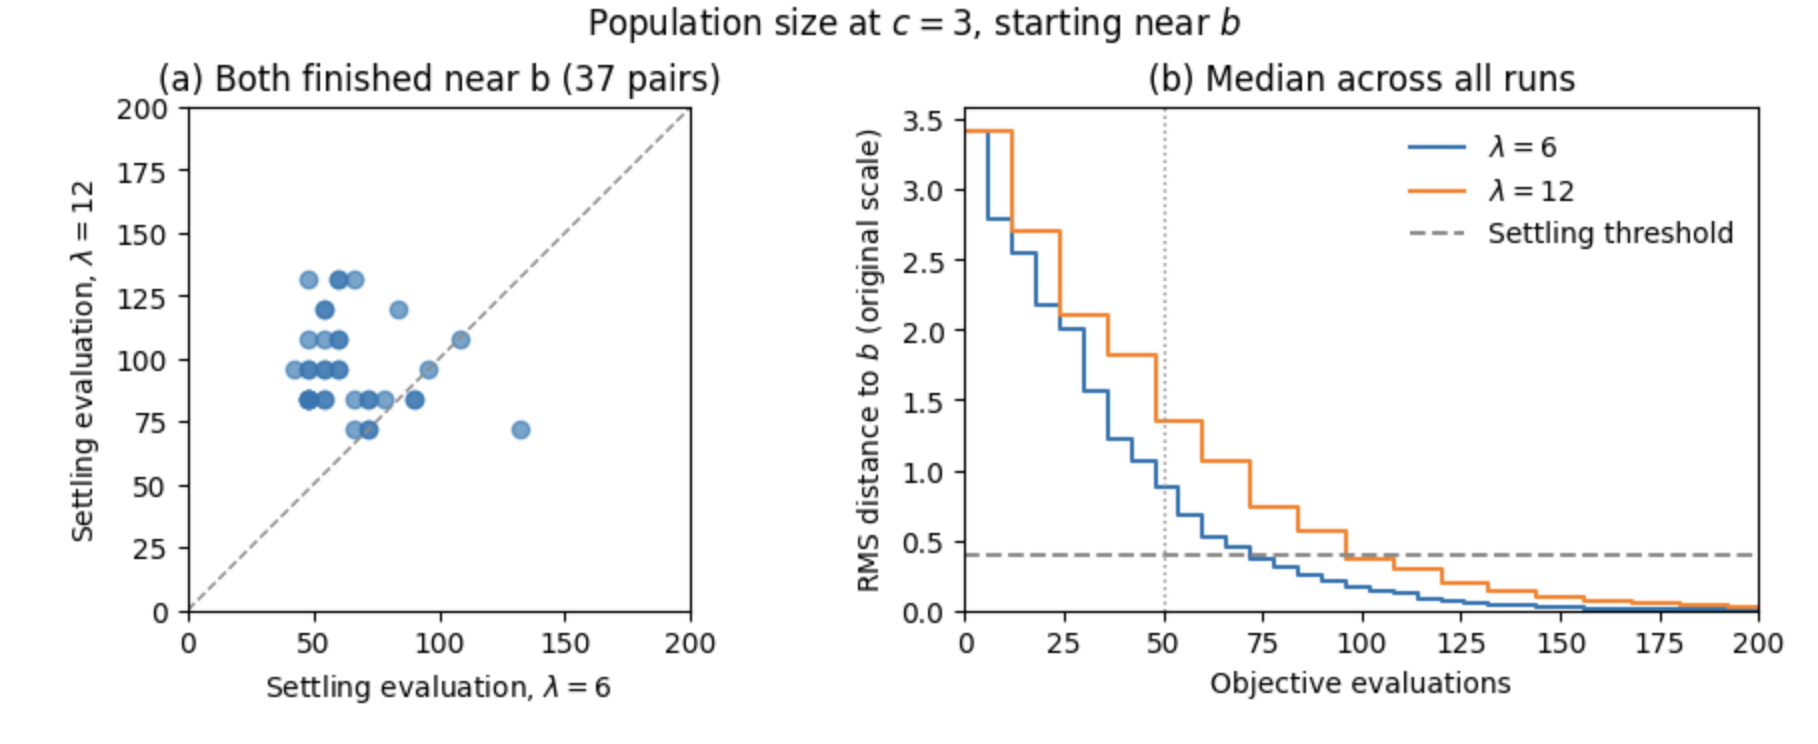
\includegraphics[width=0.78\linewidth]{1.png}\par
\smallskip
\noindent
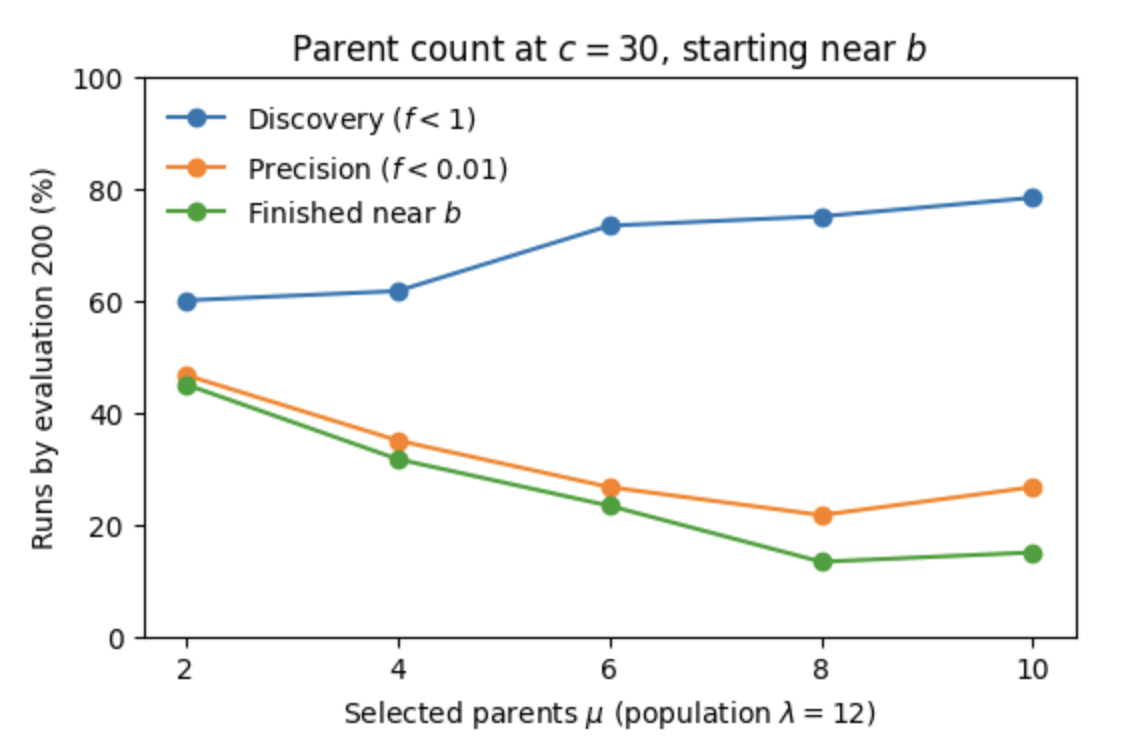
\includegraphics[width=0.36\linewidth]{2.png}\hfill
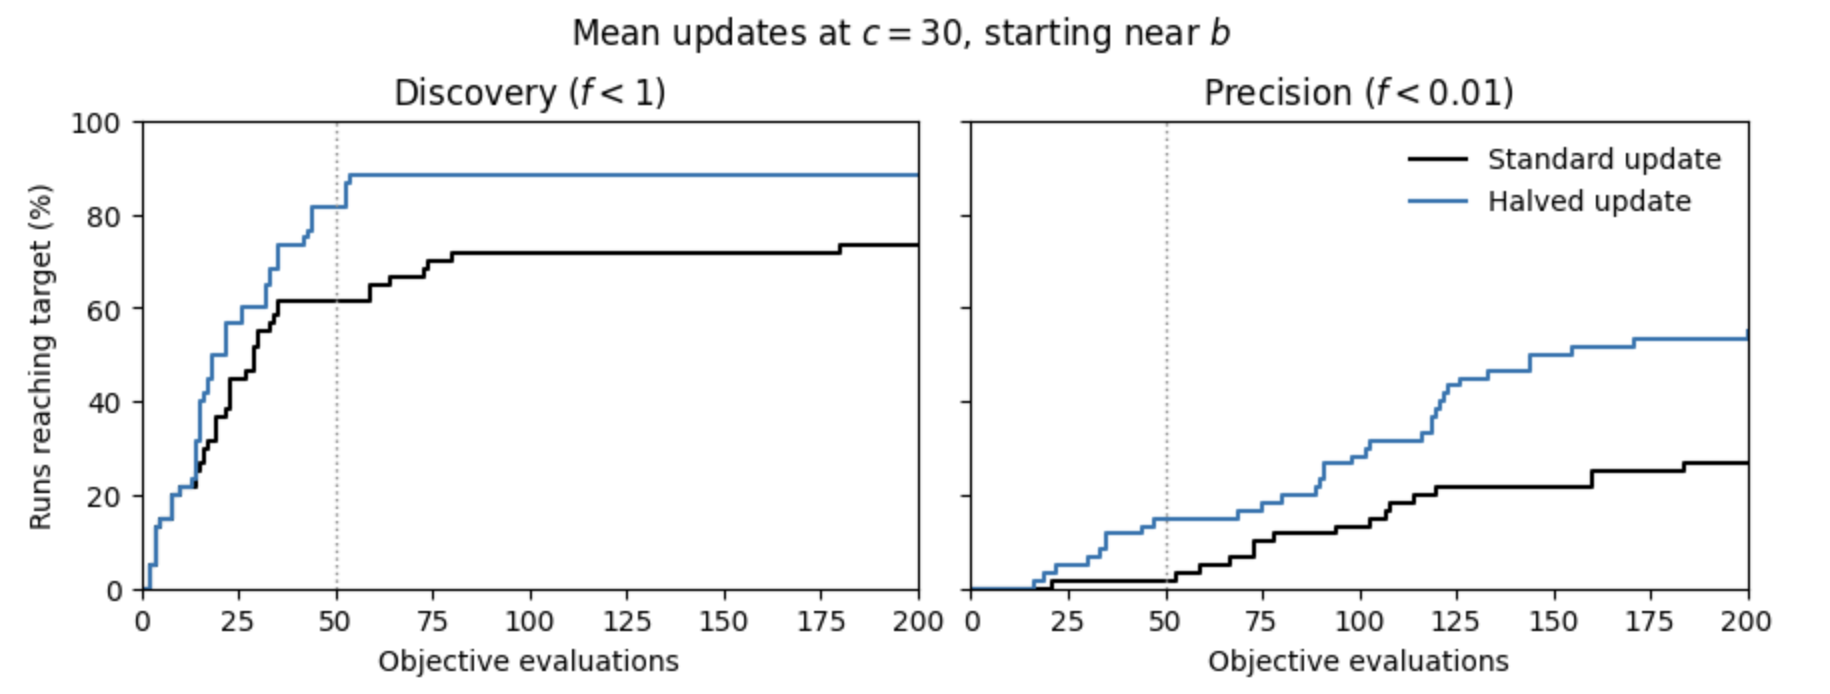
\includegraphics[width=0.61\linewidth]{3.png}\par
\caption{CMA-ES runs starting near \(b\).
The top row shows paired settling evaluations (a) and median RMS
distance to \(b\) (b) for populations of 6 and 12 at \(c=3\).
The bottom-left plot shows outcomes at evaluation 200 across parent
counts at \(c=30\) and \(\lambda=12\).
The bottom-right panel shows cumulative discovery (left) and precision
(right) for the standard and halved mean updates at \(c=30\).}
\label{fig:cmaes-results}
\end{figure}

At \(c=3\), the smaller population usually settled sooner among
pairs where both settled near \(b\), while the larger population
finished near \(b\) more often overall. At \(c=30\), the population
and parent-count comparisons
show a trade-off by 200 evaluations. The smaller configurations
yielded fewer discoveries and more precision hits. Halving the mean
update improved both outcomes when CMA-ES started near \(b\), and
the search mean ended closer to \(b\). Experiment~3 builds on this
finding by comparing BO and CMA-ES under initial designs near \(A\)
and \(B\) to test how starting information affects discovery and
refinement.




